\section{¿Qué es una demostración?}

El problema es que no se enseña a escribir textos matemáticos.
Como mucho, se exponen demostraciones delante de los alumnos, pero luego no se les exige que lo hagan bien ellos mismos hasta el último detalle y con rigurosidad.
Una demostración en matemáticas es el texto más común.
Empezaremos por revisar la estructura de una demostración y sus tipos.
Una vez aprendida la estructura de esta pieza básica de la escritura matemática, entraremos a fondo en otras cuestiones más generales tales como las refutaciones, la escritura de problemas, los principios generales de escritura y la corrección lingüística.

Una demostración o prueba está compuesta de tres partes: premisas, razonamiento y consecuencia.
Las premisas se llaman también hipótesis y la consecuencia, tesis o conclusión.
La relación entre las premisas, el razonamiento y la consecuencia es que siempre que las premisas sean ciertas y exista un razonamiento lógicamente correcto, entonces la consecuencia es cierta.
Un enunciado que relacione un conjunto de premisas y una consecuencia se llama teorema.
Probar o demostrar un teorema consiste en proporcionar un razonamiento lógicamente correcto que una premisas y conclusión.
Por ejemplo, veamos el siguiente teorema.

\begin{theorem}
    Sean $a,b,c$ tres enteros, donde $a,b \neq 0$.
    Entonces, si $a$ divide a $b$ y $b$ divide a $c$, se sigue que $a$ divide a $c$.
\end{theorem}

El teorema 1 establece que la divisibilidad es una propiedad transitiva.
La primera línea
\begin{center}
    Sean $a,b,c$ tres enteros, donde $a,b \neq 0$.
\end{center}
delimita el alcance del teorema.
Proclamamos la transitividad de una propiedad de los números enteros, pero no de otros conjuntos de números.
Esto es una cuestión de precisión.
La segunda línea
\begin{center}
    Entonces, si $a$ divide a $b$ y $b$ divide a $c$, se sigue que $a$ divide a $c$.
\end{center}
es el núcleo del enunciado del teorema, esto es, donde reside la sustancia lógica del teorema.
Las premisas son $a$ divide a $b$ y $b$ divide a $c$; la consecuencia, $a$ divide a $c$.
El teorema establece que si es cierto que $a$ divide a $b$ y $b$ divide a $c$, entonces es cierto también que $a$ divide a $c$.
Otros teoremas pueden tener una estructura lógica menos evidente.
Por ejemplo:
\begin{theorem}
    Sea $p$ un número primo y $a,b$ dos números enteros.
    Si $p$ divide a $a\cdot b$, entonces o bien $p$ divide a $a$ o bien $p$ divide a $b$.
\end{theorem}
La consecuencia del teorema 2 consiste en dos enunciados, $p$ divide a $a$ y $p$ divide a $b$, y la consecuencia establece que uno de los dos o ambos es cierto.
En este ejemplo, la estructura lógica del teorema es más complicada.
He aquí otro ejemplo de teorema.
\begin{theorem}
    Sea $n \geq 1$ un natural.
    La siguiente fórmula es cierta para todo $n$:
    \[
        1 + 2 + \cdots + n = \frac{n(n + 1)}{2}.
    \]
\end{theorem}
Aquí la estructura del teorema 3 es
\begin{center}
    Si $n\geq 1$ es un número natural, entonces\\ $1 + 2 + \cdots + n = \frac{n(n + 1)}{2}$ es una igualdad cierta.
\end{center}
a pesar de que en la redacción literal del teorema 3 la palabra “entonces” no aparece.
En general, la estructura de un teorema es
\begin{figure}[H]
    \centering
    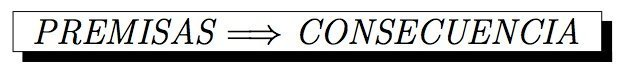
\includegraphics[width=0.6\linewidth]{images/Figura-premisas-consecuencia}\label{fig:figure}
\end{figure}
Entonces, ¿qué es un razonamiento?
Un razonamiento es una cadena de argumentos que llevan desde las premisas a la consecuencia.
El razonamiento es correcto cuando cada argumento es lógicamente correcto.
Por tanto, si el teorema es de la forma
\[
    P \implies Q
\]
donde $P$ es la premisa y $Q$ la consecuencia, la demostración es una cadena de argumentos lógicamente correctos que parte de las premisas y acaba en la conclusión, como la siguiente:
\[
    P \implies R_1 \implies R_2 \implies \ldots \implies R_k \implies Q
\]
donde cada $R_i$ es un razonamiento intermedio.
Un teorema puede ser demostrado con diferentes pruebas (unas serán más elegantes y simples que otras).
Veamos la demostración del teorema 1.
Empezamos por aplicar la definición de divisibilidad a los enteros $a$ y $b$.
\begin{proof}
    Como $a$ divide a $b$, entonces existe un entero $k_1$ tal que $b = a \cdot k_1$.
    Análogamente, como $b$ divide a $c$, existe otro entero $k_2$ tal que $c = b \cdot k_2$.
    \par\textbf{\small(La siguiente idea es combinar las dos igualdades obtenidas.)}\par
    Dado que $b = a \cdot k_1$ y $c = b \cdot k_2$, podemos sustituir $b = a\cdot k_1$ en la segunda igualdad:
    \[
        c = b \cdot k_2 = a\cdot k_1 \cdot k_2 = a\cdot (k_1 \cdot k_2).
    \]
    \textbf{\small(Finalmente, anunciamos la consecuencia del teorema, que es una consecuencia lógica del argumento.)}\par
    La igualdad $c = a \cdot (k_1 \cdot k_2)$ significa que $a$ divide a $c$.
    Por tanto, la propiedad de divisibilidad es transitiva.
\end{proof}
El símbolo \qedsymbol\ se coloca al final de una prueba para indicar su fin.
También se emplea el acrónimo QED, que en latín significa “como queríamos demostrar”.

Hay una cuestión a la que los estudiantes tienen que prestar atención: las definiciones.
Muchos estudiantes escriben demostraciones incorrectas porque no saben o no recuerdan las definiciones.
Las definiciones son términos que fijan el significado de objetos y propiedades matemáticos.
Por ejemplo, se define el valor absoluto porque es una función que aparece con suma frecuencia; en este caso, la definición se ha hecho por concisión y comodidad de uso.
En cambio, la definición de continuidad recoge una propiedad abstracta, el que límite en un punto coincida con el valor de la función.
Los términos matemáticos tienen significado diferente al que poseen en el lenguaje natural.
Antes de escribir una prueba es una buena idea revisar las definiciones pertinentes.